\section{Архитектура системы сбора данных CBM~RICH}\label{section:secReadout}

\subsection{64-канальный модуль считывания}\label{section:secModule}

Конструктивно и функционально вся электроника считывания и оцифровки данных CBM~RICH может быть сгруппирована в 64-канальные модули, каждый из которых соответствует одному многоанодному фотоэлектронному умножителю (МА~ФЭУ). Схема 64-канального модуля показана на \figref{fig:ReadoutModule}. Он включает в себя 4~платы PADIWA и одну плату TRB~v3.

\begin{figure}
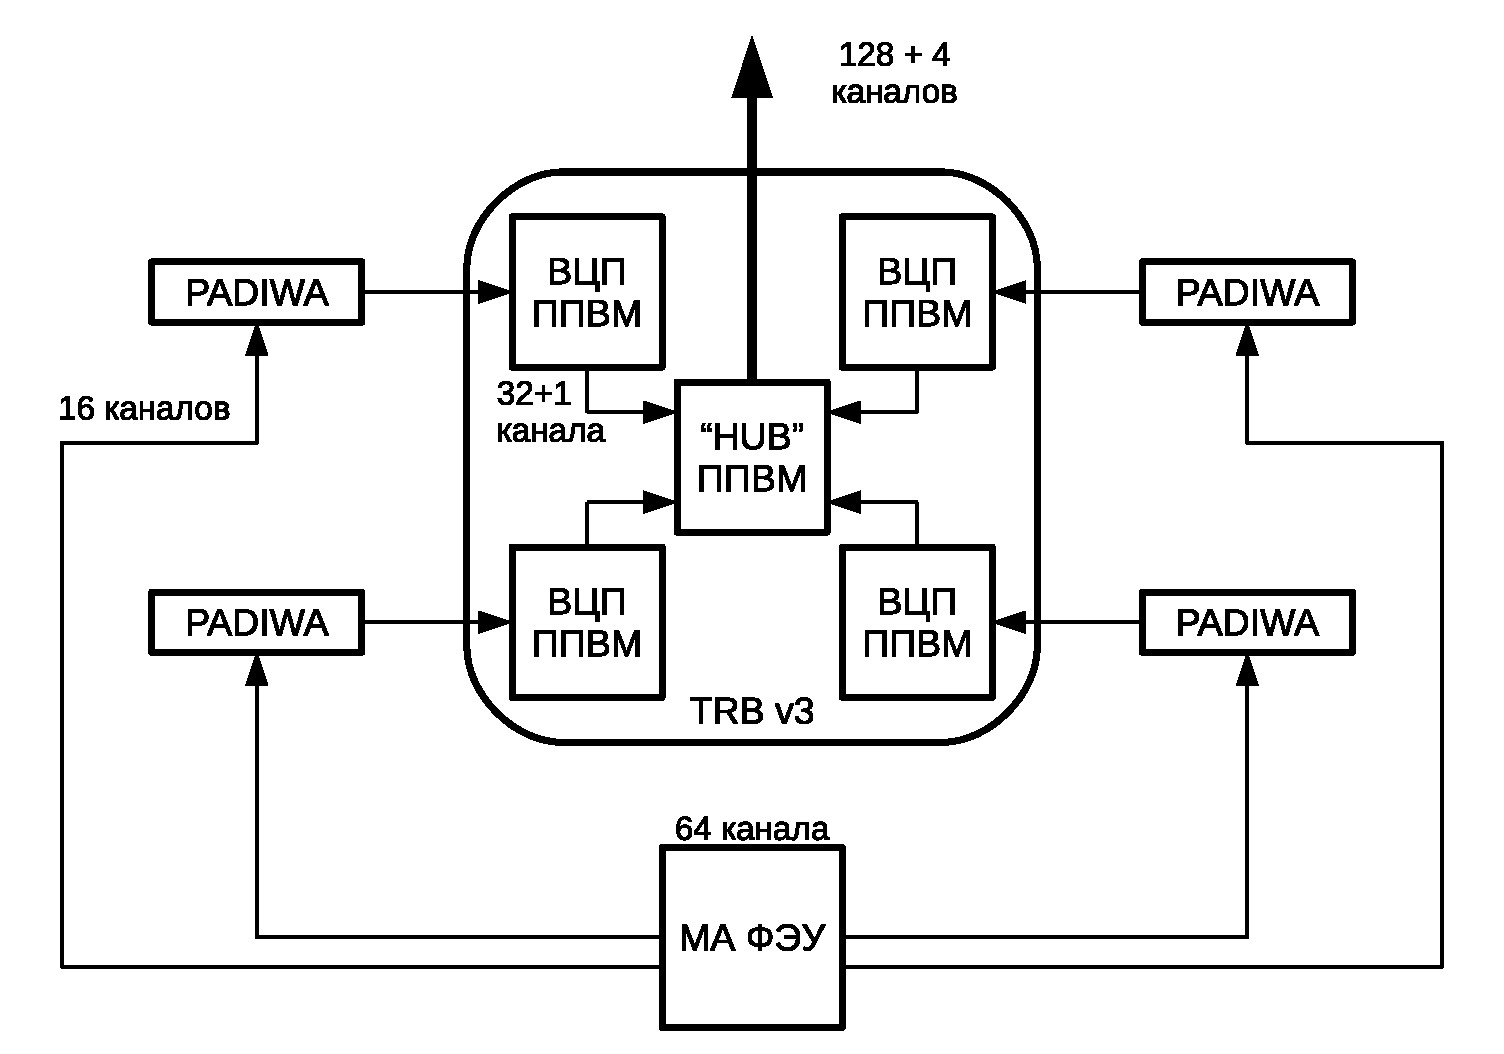
\includegraphics[width=1.0\textwidth]{pictures/4_A_PMT_readout_rus.eps}
\caption{Схема считывания одного МА~ФЭУ, состоящяя из 4~плат-дискриминаторов PADIWA и одной платы TRB~v3.}
\label{fig:ReadoutModule}
\end{figure}

PADIWA --- 16-ти канальная плата передней электроники, разработанная в ГСИ~\cite{TRBSITE}. Общий вид платы PADIWA показан на \figref{fig:PADIWA}. Плата устанавливается на МА~ФЭУ через плату-адаптер, единственным назначением которой является соединение анодов МА~ФЭУ с соответствующими входами PADIWA. С одной стороны печатной платы PADIWA расположены 16~сигнальных входов с импедансом 100~кОм. На каждый вход приходится два контакта --- земля и сигнал. Они чередуются таким образом, чтобы можно было подключить PADIWA к плате-адаптеру любой стороной. Каждый канал PADIWA имеет собственный фильтр низких частот с полосой пропускания около 100~МГц и предусилитель, которые образуют аналоговую часть канала. После усиления сигнал поступает в программируемую пользователем вентильную матрицу (ППВМ). Обычно ППВМ применяются для обработки цифровых (логических) сигналов, однако, в нашем случае на входные цифровые линии подаётся аналоговый сигнал. В ППВМ для каждой входной линии можно задать свой порог, разделяющий логические уровни входного сигнала. Таким образом, настраиваемые входы ППВМ могут использоваться как дискриминаторы. На выходе каждого канала формируется логический ноль, когда входной сигнал в этом канале ниже установленного порога, и логическая единица, когда входной сигнал выше этого порога, см.~\figref{fig:Discrimination}. Далее расположены выходные порты и порты настройки ППВМ, объединённые в разъем, позволяющий подключить 20~LVDS линий. Для управления платой используются 4~LVDS линии, остальные 16~LVDS линий --- выходные. Для программирования ППВМ на плате предусмотрен стандартный JTAG порт. Также на плате имеется порт для подключения источника низкого напряжения для питания платы. Помимо этого имеется датчик температуры, подключённый к ППВМ. Сигналы с датчика могут использоваться, например, для того, чтобы обнаружить перегрев, если такая возможность заложена в программе ППВМ.

\begin{figure}
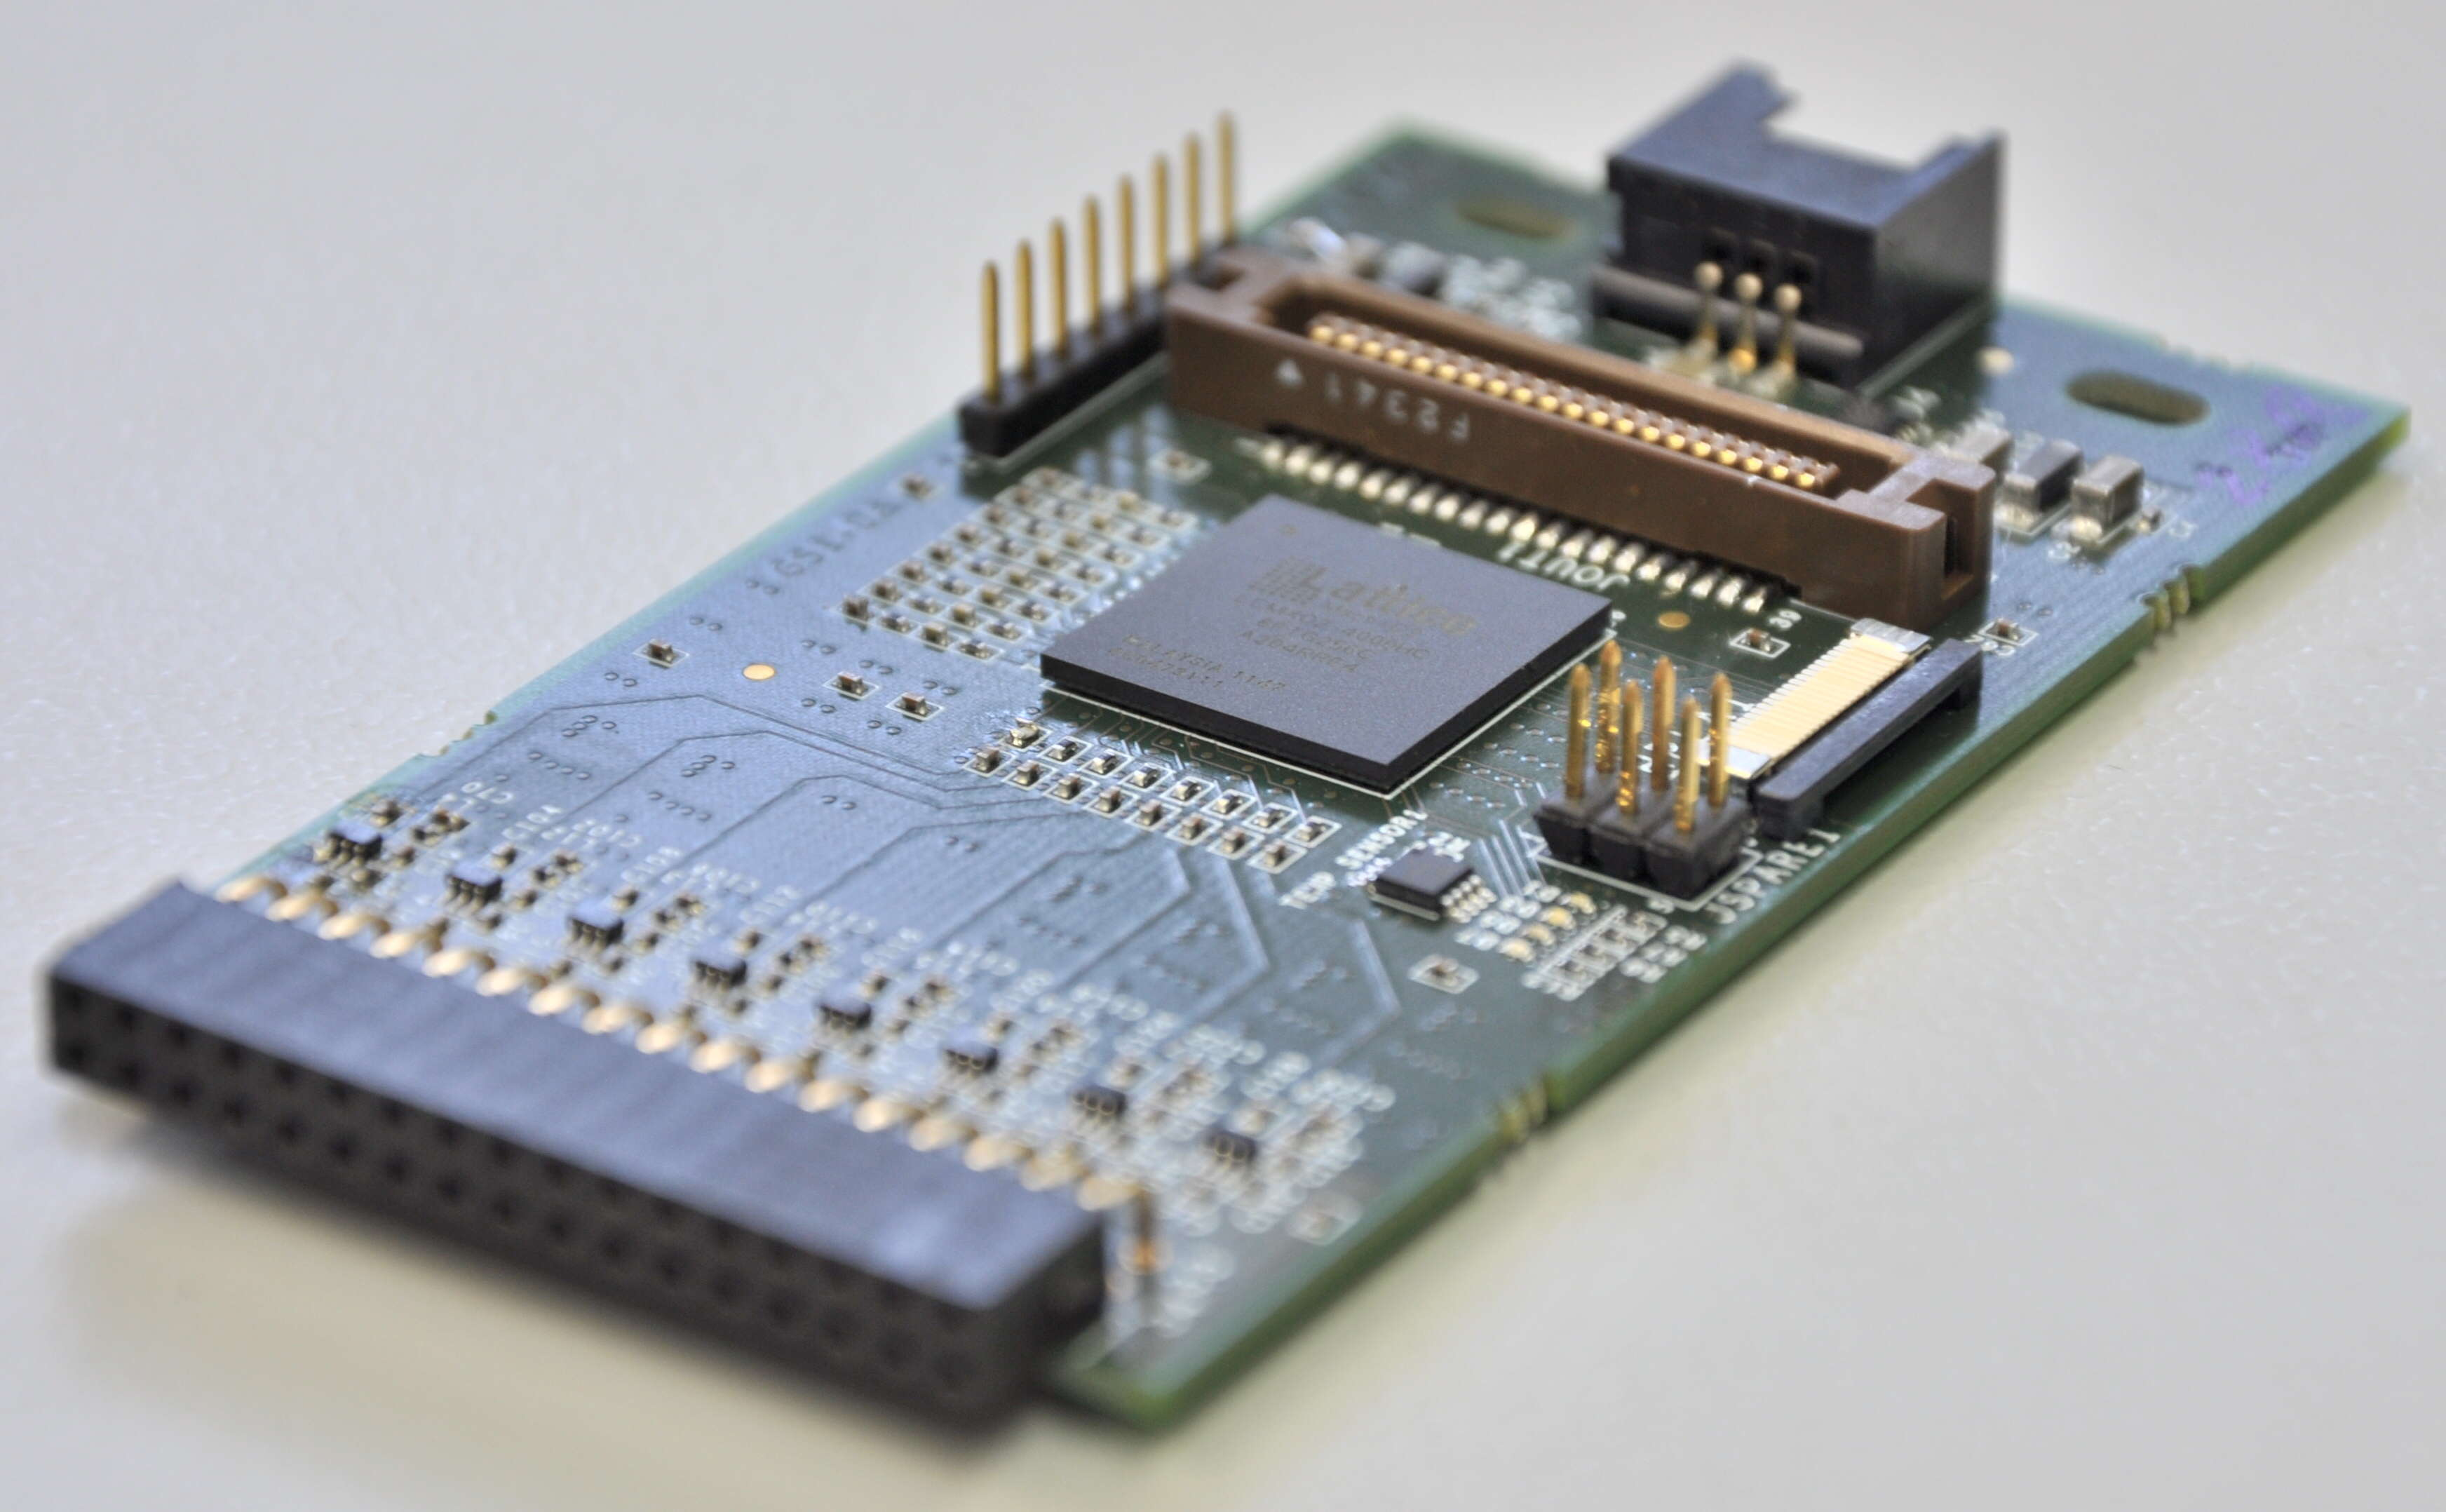
\includegraphics[width=1.0\textwidth]{pictures/5_padiwa_lowres.jpg}
\caption{Общий вид платы PADIWA.}
\label{fig:PADIWA}
\end{figure}

\begin{figure}
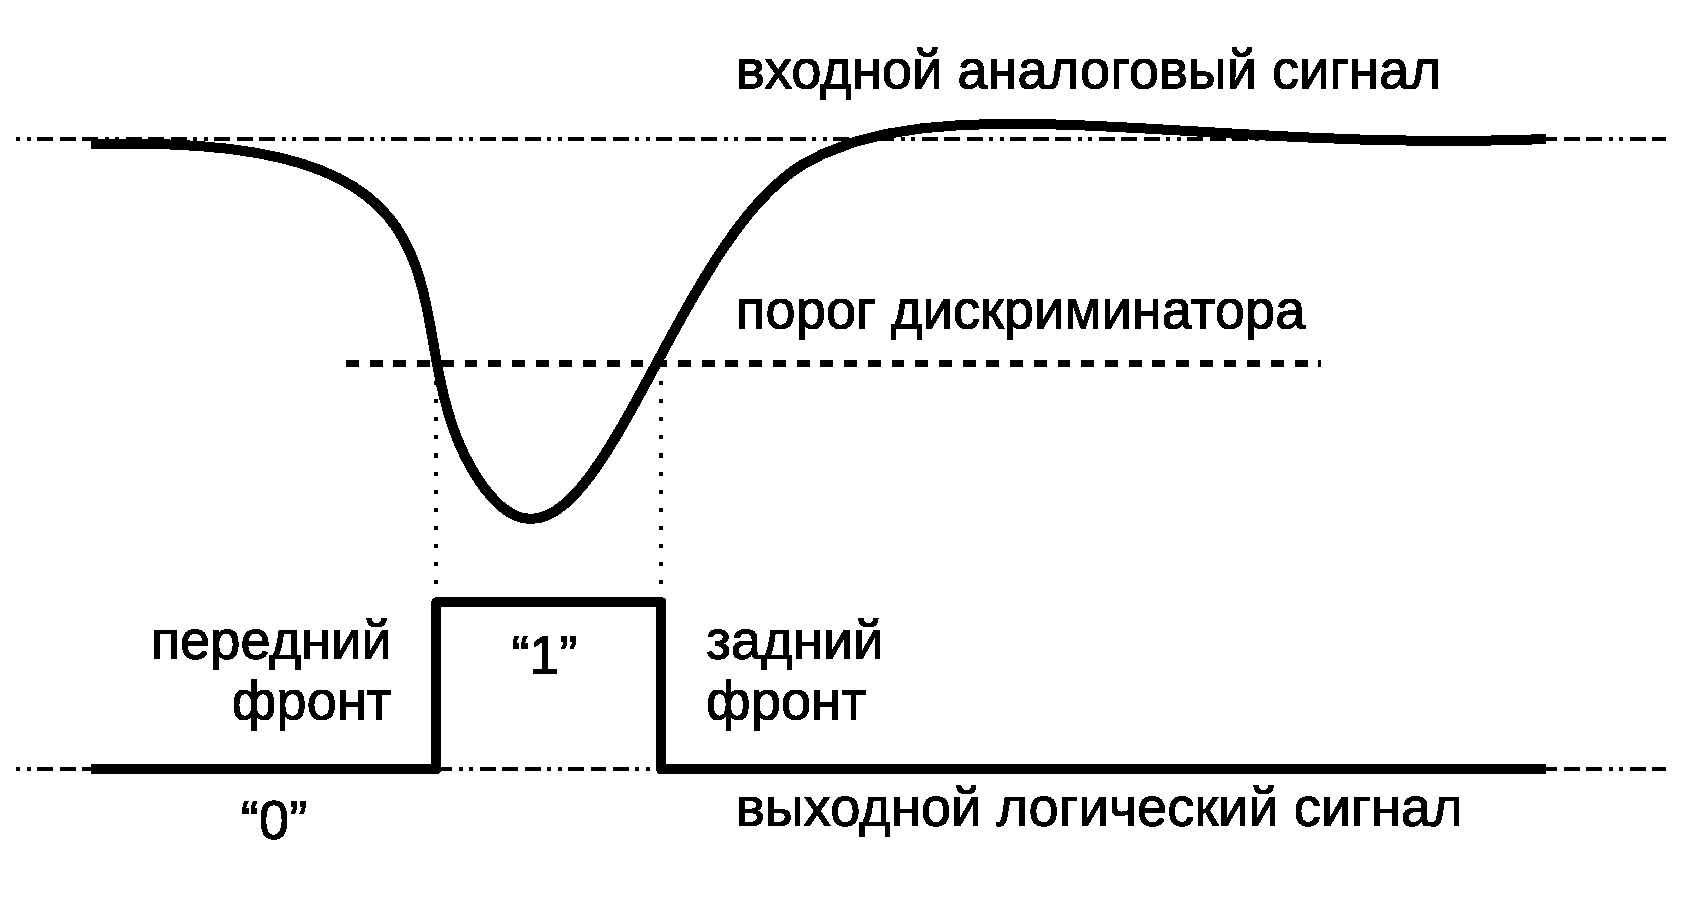
\includegraphics[width=1.0\textwidth]{pictures/6_Discrimination_rus.eps}
\caption{Условная временная диаграмма функционирования дискриминатора.}
\label{fig:Discrimination}
\end{figure}

Многофункциональная плата TRB~v3 содержит 5~ППВМ, каждую из которых можно запрограммировать независимо. Различают 1~центральную ППВМ и 4~периферийные. В нашем случае 4~периферийные ППВМ запрограммированы как время-цифровые преобразователи~(ВЦП), а центральная ППВМ --- как концентратор данных. Такую конфигурацию платы будем называть TRB~v3 (конфигурация~1).

% первый-второй либо один-другой, не так ли?
Выходные логические LVDS сигналы со всех 16~каналов платы PADIWA поступает в одну из периферийных ППВМ платы TRB~v3, где каждый входной канал разветвляется на два канала ВЦП --- один чувствителен к переднему фронту, второй --- к заднему. К получившимся 32~каналам в каждой периферийной ППВМ добавляется канал синхронизации. Таким образом, на выходе всей платы TRB~v3 имеются 132~канала.

% В частности, существует специальная плата расширения для подключения шлейфов от плат PADIWA (это и сигнал и управление, выше же описано).
Общий вид платы TRB~v3 показан на \figref{fig:TRB}. Рядом с каждой периферийной ППВМ имеются специальные порты, к которым можно присоединить платы расширения. В частности, к плате расширения подключается сигнальный шлейф от платы PADIWA. На плате TRB~v3 имеются порты Ethernet, как RG45, так и оптический SFP, которые используются для двусторонней связи с другими платами TRB~v3 или с компьютером.

\begin{figure}
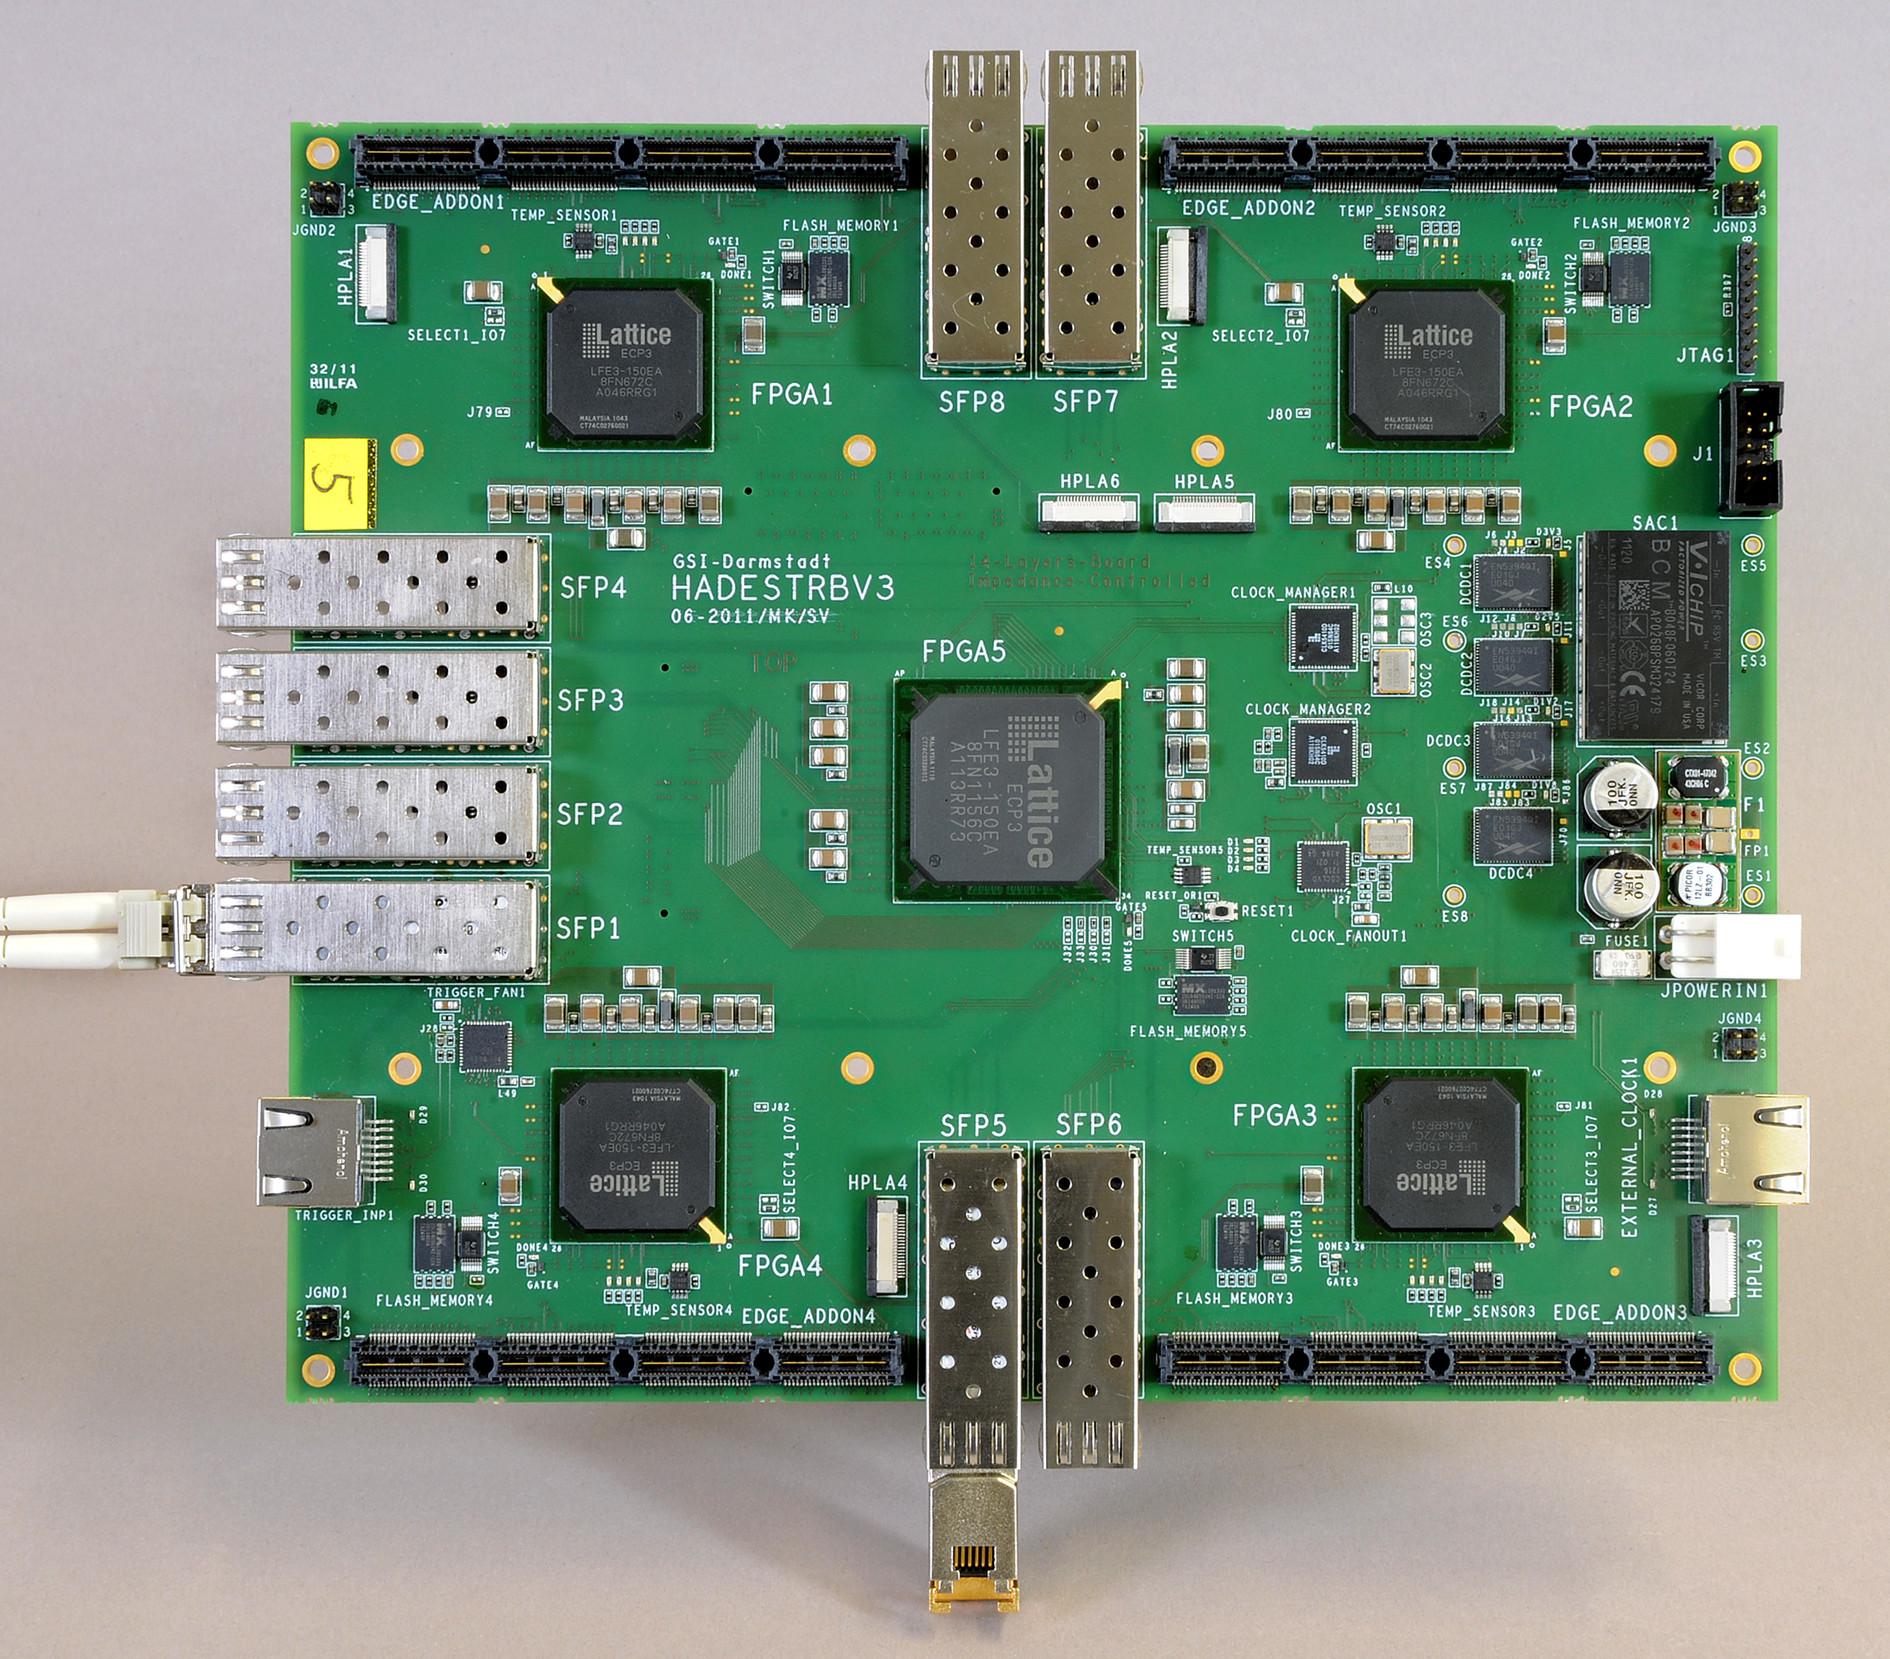
\includegraphics[width=1.0\textwidth]{pictures/7_TRB3_crop.jpg}
\caption{Общий вид платы TRB~v3.}
\label{fig:TRB}
\end{figure}

Каждая периферийная ППВМ, разбивается на 32~области, в каждой из которых программируется одна и та же схема канала ВЦП. 
% Правильное предложение?
Каналы расположены в разных областях матрицы, поэтому каждый канал ВЦП имеет свою величину пути, проходимого сигналом внутри ППВМ.
Нечетные каналы настроены на положительный перепад напряжения, т.е. на передний фронт, а четные каналы --- на отрицательный перепад напряжения, т.е. на задний фронт. Обработка импульса из одного входного канала выполняется двумя каналами ВЦП, относительная задержка между которыми должна быть прокалибрована с помощью точного генератора прямоугольных импульсов. Особенности такой калибровки обсуждаются в~\ref{}. Отметим, что в ППВМ для каждого канала ВЦП имеется специальный счётчик количества зарегистрированных временных отметок, значение которого может быть опрошено независимо от основного потока данных. Этот счётчик может быть использован, например, для получения зависимости скорости счёта от порога дискриминатора с целью определения оптимального порога.

Регистрация момента времени в ВЦП осуществляется в два этапа. Грубое значение регистрируется кольцевым счётчиком, который управляется от тактового генератора с периодом 5~нс. Старшие 28~разрядов счетчика называются эпохой (epoch), а 11~младших разрядов называются грубым временем (coarse)~\cite{}. При регистрации момента времени входного фронта значение времени кодируется двумя сообщениями --- эпохой и собственно так называемой временной отметкой (timestamp). Чтобы уменьшить поток выходных данных значение эпохи, которое увеличивается каждые 10.24~мкс, передаётся однократно для группы временных отметок, принадлежащих данной эпохе.

Для более точного измерения применяется дополнительный 10-битный регистр точного времени (fine). В регистр пишется значение счётчика точного времени, реализованного с помощью технологии Tapped delay line (TDL) на 512-ти элементах. Теоретически, если все элементы задержки идентичны, полный период счётчика грубого времени, равный 5~нс, можно разбить на 512~отсчётов. Тогда точность измеренной временной отметки была бы равна 9.9~пс, а полное время рассчитывалось бы как $ T = (epoch \cdot 2048 + coarse - (fine/512)) \cdot 5 $нс.

Однако, в силу неидеальности компонентов, существует разброс параметров элементов в линии задержки, следовательно, требуется калибровка результатов измерения точного времени относительно диапазона значений регистра. Процедура калибровки и анализ ее качества обсуждаются в секциях~\ref{section:secSoft}~и~\ref{section:FTcalib} соответственно.

Находящиеся на TRB~v3 ППВМ формируют 4-байтовые сообщения одного из следующих типов: EVENT, SUBEVENT, SUBSUBEVENT HEADER, TDC HEADER, EPOCH COUNTER, TIMESTAMP, DEBUG. Логика формирования сообщений подробно описана в документации~\cite{TRBDOCU}.

Рассмотрим для примера структуру сообщения типа TIMESTAMP, наиболее информативного для нашего анализа. В зависимости от номера канала это сообщение может нести информацию о фронте синхронизации SYNC, о переднем фронте хита LEAD или о заднем фронте хита TRAIL.

\begin{figure}
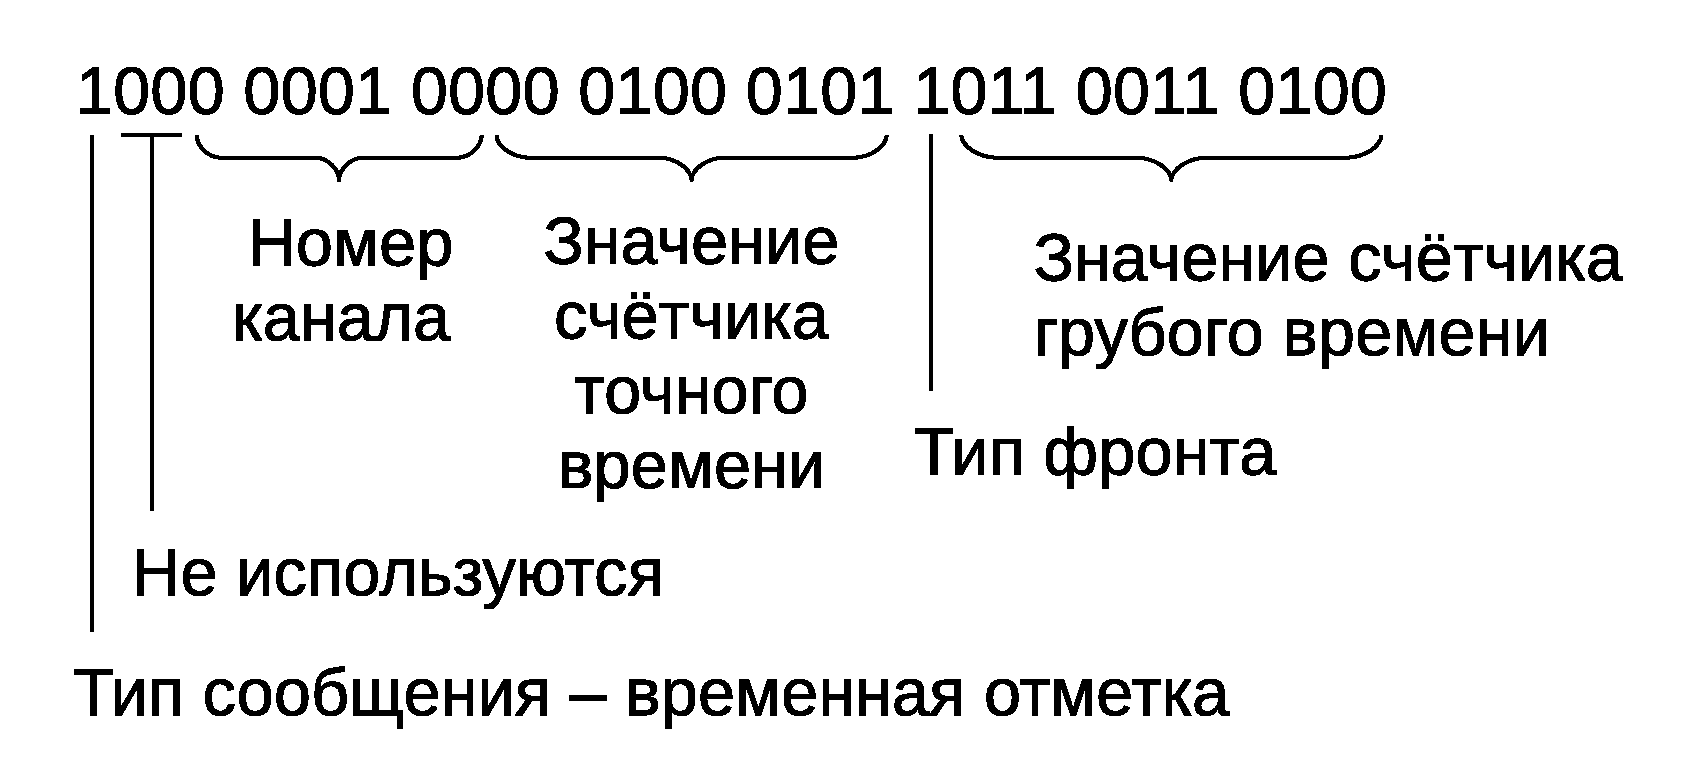
\includegraphics[width=1.0\textwidth]{pictures/8_Unpacking.eps}
\caption{Пример сырого сообщения типа ``временная отметка''.}
\label{fig:Unpacking}
\end{figure}

Старший бит (левый) указывает на то, что данное сообщение является временной отметкой. Следующие два бита не используются. Следующие 7 бит указывают номер канала 4. Затем 10 бит указывают значение счётчика точного времени 0x45. Далее вспомогательный бит edge, который на данный момент не используется. Последние 11 бит кодируют значение счётчика грубого времени 0x334. Далее отсюда вычисляется полное значение времени в наносекундах (2681319745539.841309).

Необходимо отметить, что каждый канал считывания характеризуется некоторой индивидуальной задержкой между моментом рождения фотоэлектрона и значением отметки времени переднего фронта. Эта задержка определяется временем развития электронной лавины в динодной системе, временем распространения сигнала по проводникам и временем переключения логических элементов. Процедура коррекции задержек и ее особенности описаны далее в секциях~\ref{section:secSoft}~и~\ref{section:Corrections}.

\subsection{Концентрация и ввод данных в ЭВМ}\label{section:secFinalReadout}

В концепции системы сбора данных эксперимента CBM предусмотрено 4~функциональных уровня, каждый из которых реализован соответствующими платами. В общем случае к детектору примыкает плата передней электроники (FEB --- front-end board), где осуществляются аналоговые преобразования и оцифровка сигналов. Далее, данные в виде электрических цифровых сигналов поступают в плату считывания (ROB --- readout board), где происходит концентрация данных и их пересылка по оптическому каналу. На следующем уровне расположены платы обработки данных (DPB --- data processing board). DPB уплотняют данные с различных детекторов за счет удаления избыточной информации специфическим для каждого детектора способом и группируют эти данные в пакеты, называемые срезами времени (time slice). В каждый срез времени попадают сообщения со всех детекторов, имеющие временную отметку в заданном интервале. Далее они передаются по меньшему числу оптических каналов с более высокой пропускной способностью~\cite{DPB}. После этого данные поступают в память, доступную центральному процессору ЭВМ по высокоскоростной шине через платы интерфейса, называемые FLIB. Аббревиатура FLIB обозначает FLES Interface Board, а FLES~\cite{FLES}, в свою очередь, обозначает First Level Event Selector, т.е. специализированный аппаратно-программный комплекс для построения событий ``на лету'' и их отбора по заданным критериям. Плата FLIB может быть реализована, например, путем программирования коммерческой PCI-E платы HTG~K-7.
%Ссылка

В случае пучковых тестов RICH плата передней электроники реализована как пара PADIWA-TRB~v3 (конфигурация~1). В будущем планируется объединение функционала этих плат на одной плате DIRICH~\cite{DIRICH}. В качестве ROB используется плата TRB~v3, сконфигурированная как концентратор. Плата DPB находится в стадии разработки прототипа, а плата FLIB была впервые применена в одном из протестированных вариантов системы сбора данных. При этом значительная часть измерений была выполнена с использованием стабильной системы сбора данных на основе DABC~\cite{DABC} и обычной сетевой карты.
